%**8-page Report Framework**
%
%1. Abstract (emphasize our variants)
%2. Introduction & Related Works (1 page)
%3. Formulation (1 page)
%4. Feature Extraction (2 pages)
%5. Learning (0.5 page)
%6. CRF Inference (0.5 page)
%7. Pixel Level result presentation (1 page)
%8. Result evaluation in rectangle level (1 page)
%9. Discussion (existing flaws and possible improvements) (0.5 page)
%10. acknowlegement and reference (0.5 page)
%
\documentclass[10pt,twocolumn,letterpaper]{article}

\usepackage{iccv}
\usepackage{times}
\usepackage{epsfig}
\usepackage{graphicx}
\usepackage{amsmath}
\usepackage{amssymb}

\DeclareMathOperator*{\argmin}{arg\,min}
\DeclareMathOperator*{\argmax}{arg\,max}
\newcommand{\SUM}{\sum\limits}
\newcommand{\hs}{\hspace{0.58in}}
\newcommand{\BOLD}{\textbf}
% Include other packages here, before hyperref.

% If you comment hyperref and then uncomment it, you should delete
% egpaper.aux before re-running latex.  (Or just hit 'q' on the first latex
% run, let it finish, and you should be clear).
\usepackage[pagebackref=true,breaklinks=true,letterpaper=true,colorlinks,bookmarks=false]{hyperref}

\iccvfinalcopy % *** Uncomment this line for the final submission
\def\iccvPaperID{****} % *** Enter the ICCV Paper ID here
\def\httilde{\mbox{\tt\raisebox{-.5ex}{\symbol{126}}}}

% Pages are numbered in submission mode, and unnumbered in camera-ready
\ificcvfinal\pagestyle{empty}\fi
\begin{document}

%%%%%%%%% TITLE
\title{Application of Conditional Random Fields to Pixel-Level Salient Object Detection Through Local, Regional and Global Features}
%\title{Application of Conditional Random Field in Image Salient Object Detection\\ with Local, Regional and Global Feature Extraction}

\author{Jimmy Lin\\
Australian National University\\
Canberra, Australia\\
{\tt\small \url{linxin@gmail.com}}
% For a paper whose authors are all at the same institution,
% omit the following lines up until the closing ``}''.
% Additional authors and addresses can be added with ``\and'',
% just like the second author.
% To save space, use either the email address or home page, not both
\and
Christopher Claou\'e-Long\\
Australian National University\\
Canberra, Australia\\
{\small\url{u5183532@anu.edu.au}}
}

\maketitle
% \thispagestyle{empty}

%%%%%%%%% ABSTRACT
\begin{abstract}
Making use of OpenCV, DARWIN and the MSRA dataset, we detect the saliency of an object in an image by extracting local, regional and global features at the pixel level, then combine those features with pre-fitted weights derived by logistic regression. A conditional random field is then constructed to capture the spatial continuity of the salient object, with a weighting ratio of combined unary and pairwise terms that is determined by cross-validation. The binary mask inferred by the conditional random field is then used to output a single bounding rectangle around a salient area through a winner-takes-all algorithm to label the detected salient object, by which the performance of our approach is evaluated through mean boundary displacement error. 
\end{abstract}

%% Introduction & Related Works (1 page)
\section{Introduction and Motivation}

A long-standing problem in the field of computer vision is how to calculate the saliency of objects in an image, that is, their prominence in the image when compared to their background and surrounds.  Human vision can accomplish this quite easily, since the human brain has mechanisms to direct attention to the main objects in the perceived image.  This ability has been studied by researchers in multiple fields, from physiology and psychology, to computer science.  The property of detecting a salient object is important for the latter because it leads to the ability to single out individual areas of an image, for example in automatic image cropping and vision simulation in robotics, as well as 3D surface reconstruction in augmented reality displays.  Salient object detection is still a field of active research, with multiple avenues being currently researched.
%\BOLD{CONTINUE? This leads on nicely to the next part}

\begin{figure}[h]
\begin{center}
    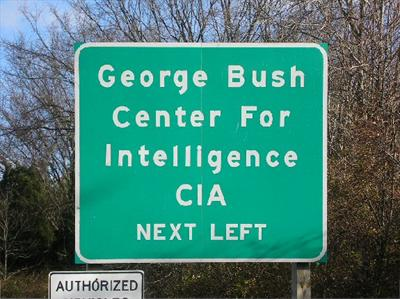
\includegraphics[width=0.6in,height=0.4in]{./Figures/example_image/4_140_140907.jpg}
    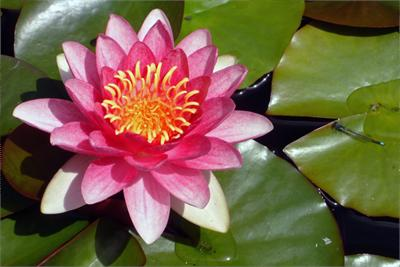
\includegraphics[width=0.6in,height=0.4in]{./Figures/example_image/4_141_141474.jpg}
    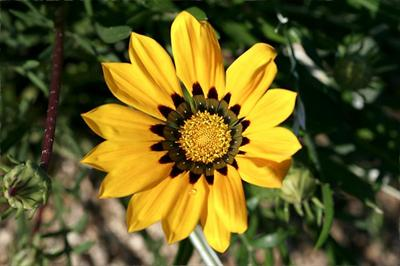
\includegraphics[width=0.6in,height=0.4in]{./Figures/example_image/4_141_141906.jpg}
    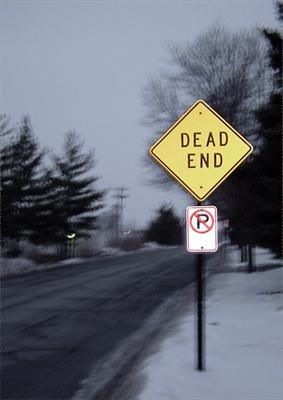
\includegraphics[width=0.6in,height=0.4in]{./Figures/example_image/4_142_142237.jpg}
    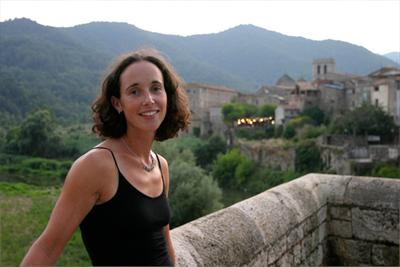
\includegraphics[width=0.6in,height=0.4in]{./Figures/example_image/4_142_142635.jpg}\\
    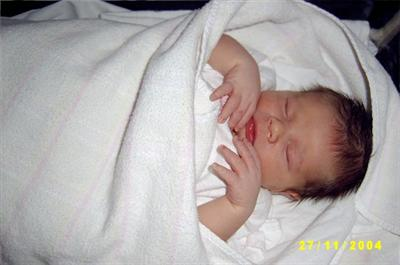
\includegraphics[width=0.6in,height=0.4in]{./Figures/example_image/4_124_124377.jpg}
    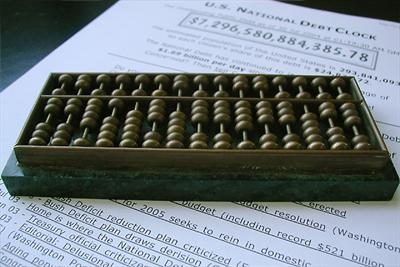
\includegraphics[width=0.6in,height=0.4in]{./Figures/example_image/4_124_124385.jpg}
    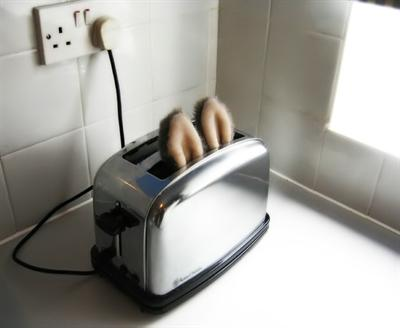
\includegraphics[width=0.6in,height=0.4in]{./Figures/example_image/4_124_124475.jpg}
    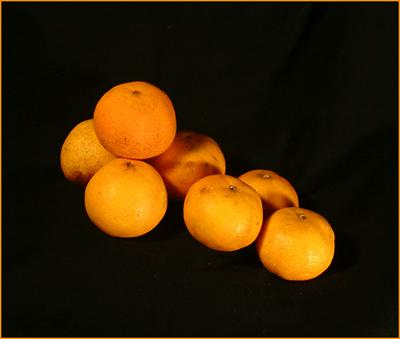
\includegraphics[width=0.6in,height=0.4in]{./Figures/example_image/4_124_124483.jpg}
    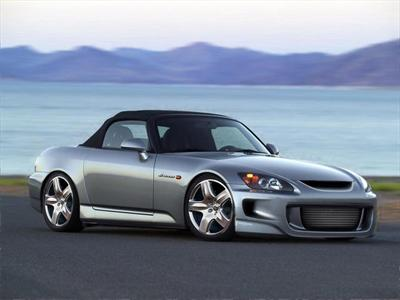
\includegraphics[width=0.6in,height=0.4in]{./Figures/example_image/4_128_128511.jpg} \\
    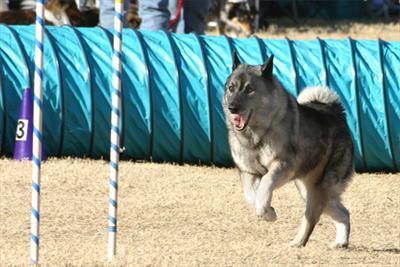
\includegraphics[width=0.6in,height=0.4in]{./Figures/example_image/4_129_129409.jpg}
    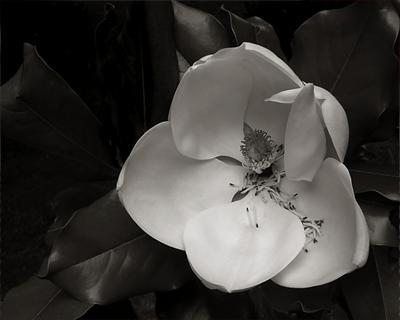
\includegraphics[width=0.6in,height=0.4in]{./Figures/example_image/4_132_132238.jpg}
    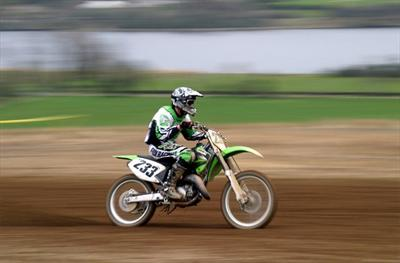
\includegraphics[width=0.6in,height=0.4in]{./Figures/example_image/4_135_135774.jpg}
    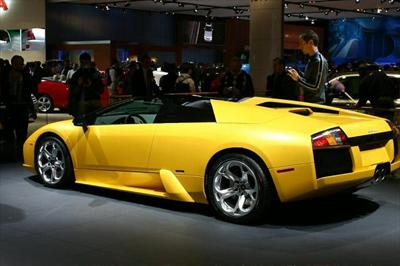
\includegraphics[width=0.6in,height=0.4in]{./Figures/example_image/4_136_136057.jpg}
    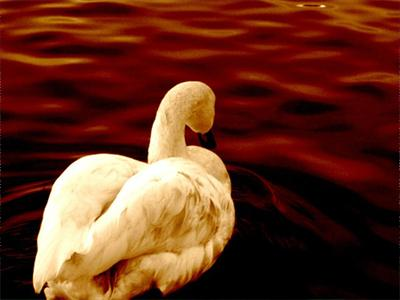
\includegraphics[width=0.6in,height=0.4in]{./Figures/example_image/4_136_136687.jpg}\\
    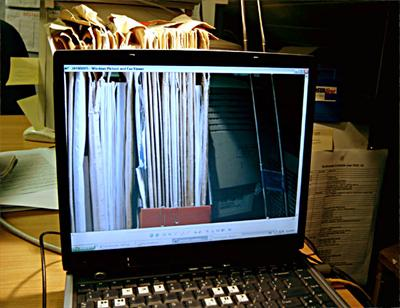
\includegraphics[width=0.6in,height=0.4in]{./Figures/example_image/4_137_137444.jpg}
    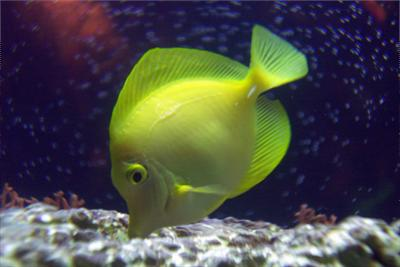
\includegraphics[width=0.6in,height=0.4in]{./Figures/example_image/4_138_138371.jpg}
    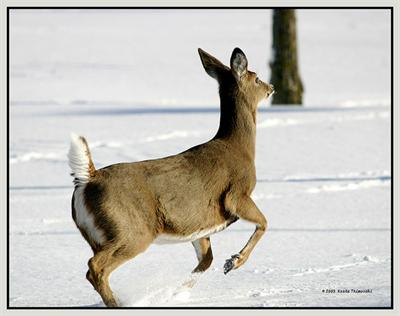
\includegraphics[width=0.6in,height=0.4in]{./Figures/example_image/4_139_139245.jpg}
    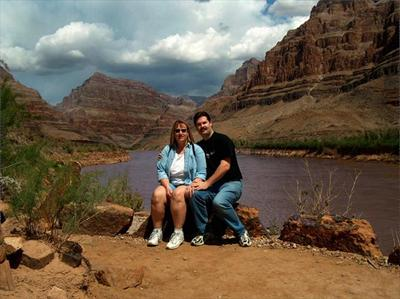
\includegraphics[width=0.6in,height=0.4in]{./Figures/example_image/4_139_139680.jpg}
    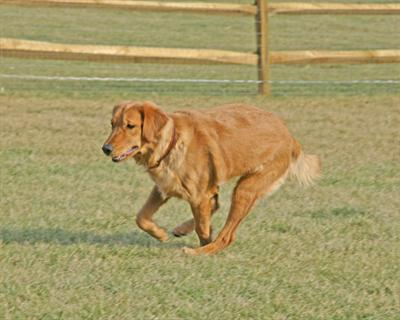
\includegraphics[width=0.6in,height=0.4in]{./Figures/example_image/4_140_140285.jpg}\\
    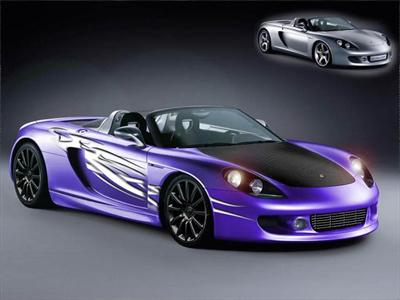
\includegraphics[width=0.6in,height=0.4in]{./Figures/example_image/4_142_142916.jpg}
    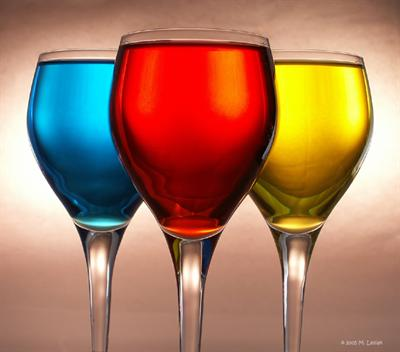
\includegraphics[width=0.6in,height=0.4in]{./Figures/example_image/4_143_143262.jpg}
    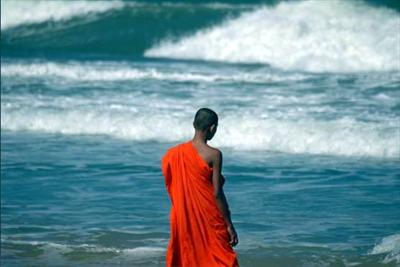
\includegraphics[width=0.6in,height=0.4in]{./Figures/example_image/4_144_144604.jpg}
    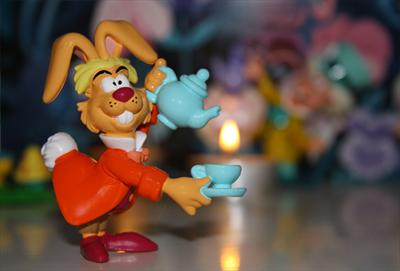
\includegraphics[width=0.6in,height=0.4in]{./Figures/example_image/4_134_134777.jpg}
    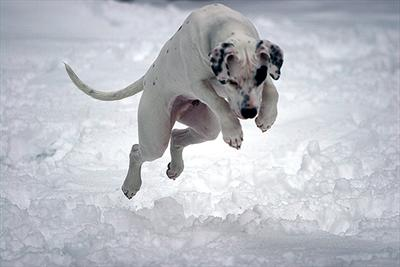
\includegraphics[width=0.6in,height=0.4in]{./Figures/example_image/4_134_134664.jpg}\\
    \caption{Example images from MSRA dataset B} \label{fig:MSRA}

    \end{center}
\end{figure}

%% Related Works (0.5 page)
\section{Related Works}
Most existing approaches are based on a bottom-up computational framework, where the computer's simulation of visual attention is driven by low-level stimuli in the scene \cite{ittiphd}\cite{itti}\cite{fuzzy}. These approaches employ three steps, the first of which is feature extraction.  Multiple low-level visual features such as intensity, colour, orientation, texture, and motion are extracted from the image at multiple scales and are then incorporated into a framework to aid in the detection of the salient object.

The second step is saliency computation. The saliency is computed by a centre-surround operation, self-information, or graph-based random walk using multiple features. After normalisation and linear/nonlinear combination, a master or saliency map is computed to represent the saliency of each pixel in the image. 

Finally, a few key locations on the saliency map are identified by winner-take-all, inhibition-of-return, or other nonlinear operations and output as a label designating the salient area in the image.

%% Formulation (1 page)
\section{Our Approach}
In our approach, we use the open source DARWIN machine learning framework \cite{drwn} as the basis for our code. We employ the MSRA dataset as the base images for our salient object detection, and build an algorithm using several suppositions that relate to how human vision differentiates salient objects from the rest of the perceived field of view.  People naturally pay more attention to salient objects in images, such as a person, a face, a car, an animal, or a road sign (Figure \ref{fig:MSRA}). This attention can be mimicked in computer vision through several factors, which were brought forward by Liu et. al in their research \cite{sal2007}\cite{sal2011}.

First of all, it is likely that pixels with a high contrast difference to their near neighbours to be part of a salient object, since they could represent a contour or boundary around an object.  This is similar to how the human brain discovers boundaries between objects in its visual field by detecting differences in light intensity.

Salient objects are more often than not quite distinct from their local surrounding region.  Calculating the distance between an object and its surrounds can therefore give us information about how salient that object is.  If we apply this concept over the entire image, we can gather information about how different various areas are to their surrounds and work out the likelihood that parts of an image are salient.

Finally, humans perceive object prominence through how distinctly coloured they are compared to the rest of the visual field.  Salient objects often demonstrate a marked difference in colour to the rest of a scene.  Therefore, the more widely distributed a colour is in an image, the less likely it is that the salient object will contain that colour.  This global colour distribution can therefore be used to describe the saliency of the pixels in an image.

\subsection{Formulation}

To turn the problem of salient object detection into a mathematical formulation, we incorporate these three high-level concepts of a salient object into the process of creating a saliency map.  Salient object detection can be formulated this way as a binary labelling task that separates a salient object from the background through multiple operations.

For each pixel $x$ of given an image $I$, the binary mask $A_x$ must indicate whether it belongs to the salient object (1) or not (0). Our objective is to compute this mask $A$ in order to show the location of the salient object in the image.

To do this, we build up a probabilistic model $$P(A|I)=\frac{1}{Z}e^{-E(A|I)}$$ to determine the probability of a binary mask over an image with $\frac{1}{Z}$ as the normalising factor, and $E(A|I)$ as an energy function incorporating both unary and pairwise potentials between pixels in the image

\begin{figure}[h]
    \begin{center}
        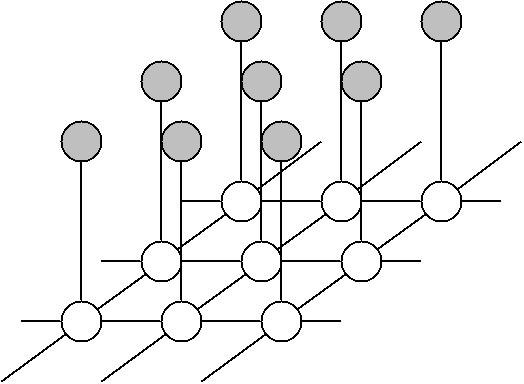
\includegraphics[width=1.8in,height=1in]{./Figures/mrf.jpg} \\
        \caption{A Conditional Random Field }
        \small White nodes are binary saliencies, grey nodes are composed features
        \end{center}
\end{figure}

Formally, the energy function can be represented as $$E(A|I) = \SUM_x S_{unary}(a_x,I) + \lambda_0 \SUM_{x,x'}S_{pair}(a_x,a_{x'},I)$$ where $\lambda$ is the relative weight between the sum of multiple unary  and pairwise features. 

The unary potential, combining the three pixel features, is specified as $$S_{unary}(a_x,I) = \SUM_{k=1}^K \lambda_k \cdot F_k(a_x,I)$$ where $\lambda_k$ is the  weight of the $k^{th}$ feature such that $\sum_{k=1}^{K} \lambda_k = 1$.

The pairwise feature $S(a_x,a_{x'},I)$ exploits the spatial relationship between two adjacent pixels.  It can be viewed as a ``penalty'' for labelling adjacent pixels differently: $$S(a_x,a_{x'},I) = |a_x-a_{x'}| \cdot e^{-\beta d_{x,x'}}$$ where $x,x'$ represent two adjacent pixels, $d_{x,x'}$ is the L2-norm (standard norm) representing the colour difference between the two pixels, and $\beta=(2\langle||I_x-I_{x'}||^2\rangle)^{-1}$ is a robust parameter to weight the colour contrast.

\begin{figure}[h]
    \begin{center} %% image 5_156_156422
    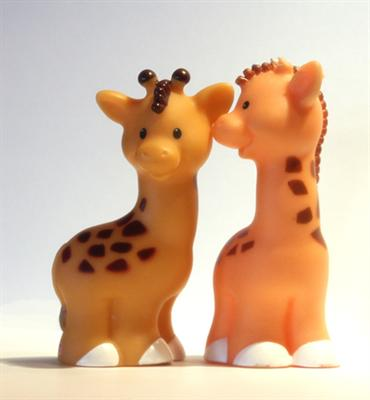
\includegraphics[width=0.6in,height=0.8in]{./Figures/previews/raw.jpg}
    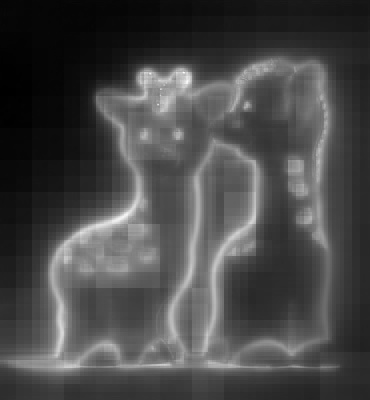
\includegraphics[width=0.6in,height=0.8in]{./Figures/previews/MC.jpg}
    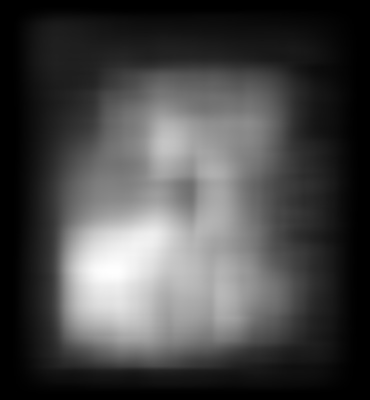
\includegraphics[width=0.6in,height=0.8in]{./Figures/previews/CSH.jpg} 
    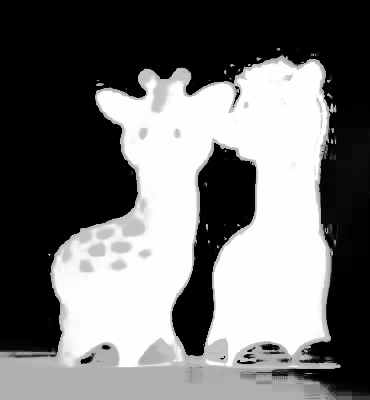
\includegraphics[width=0.6in,height=0.8in]{./Figures/previews/CSD.jpg} 
    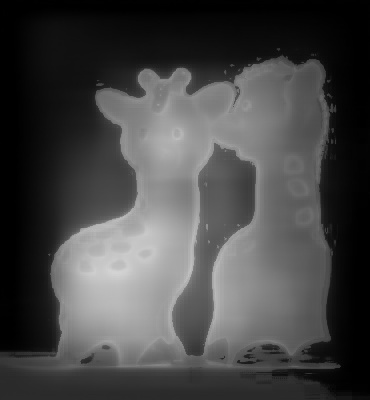
\includegraphics[width=0.6in,height=0.8in]{./Figures/previews/Composed.jpg} \\
    \caption{Original Image and Preview of feature maps}\vspace{1mm}
       \small Left to Right: Original Image, Multiscale Contrast Map, Centre-Surround Histogram, Colour Spatial Distribution, Composed Unary Potentials
\end{center}
\end{figure}

The final energy to which each feature $F_k(a_x,I)$ contributes comes from a normalised feature map $f_k(x,I)\in[0,1]$, where for each pixel: $$F_k(a_x,I) = \left\{\begin{matrix}f_k(x,I), & a_x=0\\1-f_k(x,I), & a_x=1\end{matrix}\right.$$ where we penalise the saliency quantity $f_k(x,I)$ of one pixel $x$ when that pixel was predicted not to be within the salient object ($a_x = 0$) and vice versa.


%% Feature Extraction (2 pages)
\subsection{Feature Extraction}
Feature Extraction, widely acknowledged as the most significant component of a computer vision task, represents how we want the computer to interpret raw images. In this project, we focus on three features capable of capturing saliency individually but in different levels of scope. They are respectively multiscale contrast, centre-surround histograms  and colour-spatial distribution.

Because of the time expense required to calculate these features on an image, our approach caches the feature maps of each image and uses them for both training and testing.
%% local feature
\subsubsection{Multiscale Contrast}

Constrast is commonly used as local feature because it simulates the human visual receptive fields. It acts on the fact that the boundary of salient objects tend to have a marked contrast to the surrounding region. Since we may have no prior knowledge about the size of salient object, we compute the contrast at multiple scales to then incorporate back into one map, since this will demarcate the various boundaries in the image.  This multiscale contrast map is thus a linear combination of image contrast at all levels of an N-level gaussian image pyramid, using the pixels $x$ in the image $I$.  Formally, this amounts to calculating $$f_c(x,I) = \SUM_{n = 1}^{N}\SUM_{x'\in W(x)}||I^n(x)-I^n(x')||^2$$ where W(x) is a window that delineates which area to consider as neighbouring pixels to compare contrast values.  The resulting map highlights the edges of different objects in the image, giving high prominence to the contours around the salient object.

%\BOLD{TODO ADD more technical analysis about why we should have multiple scales.}

\begin{figure}[ht]
\begin{center}    
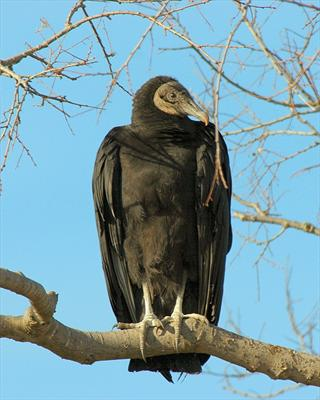
\includegraphics[width=0.65in,height=0.9in]{./Figures/pyramid/5_145_145839raw.jpg} \hspace{2mm}
 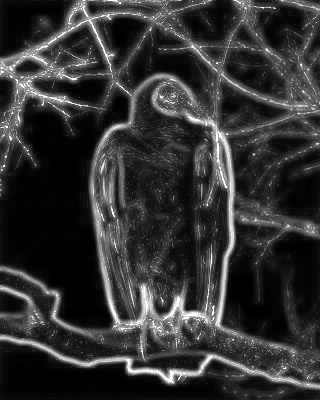
\includegraphics[width=0.65in,height=0.9in]{./Figures/pyramid/5_145_145839_p0.jpg} 
 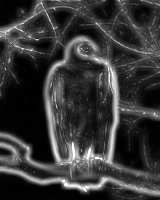
\includegraphics[width=0.325in,height=0.45in]{./Figures/pyramid/5_145_145839_p1.jpg} 
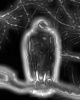
\includegraphics[width=0.1625in,height=0.225in]{./Figures/pyramid/5_145_145839_p2.jpg} 
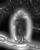
\includegraphics[width=0.08125in,height=0.1125in]{./Figures/pyramid/5_145_145839_p3.jpg} 
 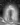
\includegraphics[width=0.040625in,height=0.0575in]{./Figures/pyramid/5_145_145839_p4.jpg} 
 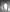
\includegraphics[width=0.0203125in,height=0.02825in]{./Figures/pyramid/5_145_145839_p5.jpg} \hspace{1mm}
 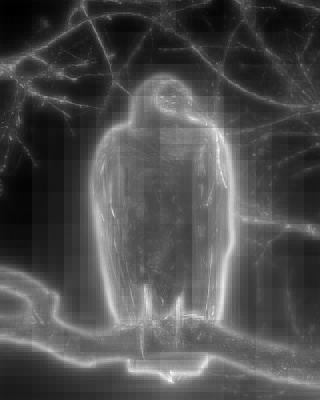
\includegraphics[width=0.65in,height=0.9in]{./Figures/pyramid/5_145_145839.jpg} \\   
\caption{Multiscale Contrast.}\small{Left: Original Image. Right: Multiscale Feature Map. \\
Middle: multiscale image pyramid from level $1$ to $6$.} \label{fig:multiscale}
\end{center}
\end{figure}


In our implementation, we choose the total number of pyramid level $N$ to be $6$ and the size of the window to be $9 \times 9$. 

As can be seen in Figure \ref{fig:multiscale}, the derived multiscale contrast map provides a highly accurate distinction between boundary and non-boundary pixels. This provides us a precise description of where the boundary of a salient object could exist in the output binary mask. When a salient object also has high contrast inside its boundaries, this feature also manages to capture the inside of the salient object, such as the bird in Figure \ref{Fig:LocalFeatureMap}(b) and the house in Figure \ref{Fig:LocalFeatureMap}(c).

But there are some drawbacks that are tough to avoid. The boundaries of all objects are highlighted, which is not desirable when searching for a single salient object.  This is because we need to give a high probability to marking pixels that are relevant to the salient object rather than every boundary possible. If this doesn't happen, there is the possibility of a "saliency leak" into non-salient areas of the final result that could deteriorate the detector's precision.


\begin{figure}[h]
    \begin{center}
    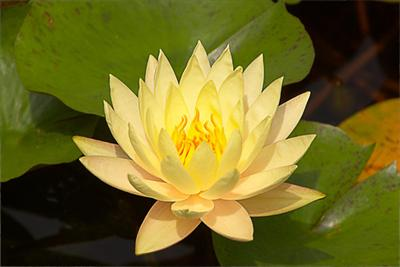
\includegraphics[width=0.7in,height=0.54in]{./Figures/contrast/1orig.jpg}
    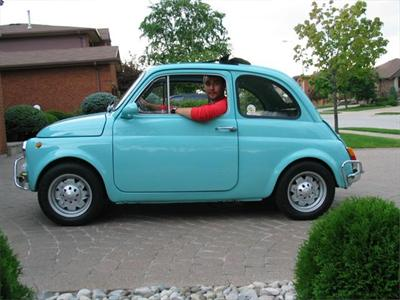
\includegraphics[width=0.7in,height=0.54in]{./Figures/contrast/2orig.jpg}
    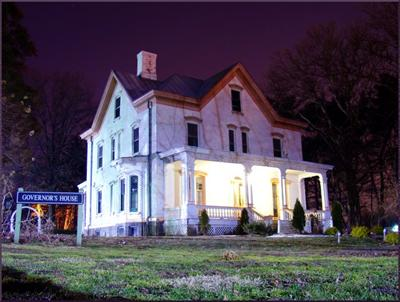
\includegraphics[width=0.7in,height=0.54in]{./Figures/contrast/3orig.jpg}
    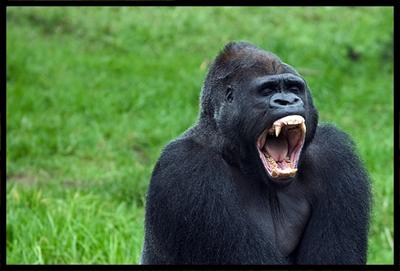
\includegraphics[width=0.7in,height=0.54in]{./Figures/contrast/4orig.jpg}\\
    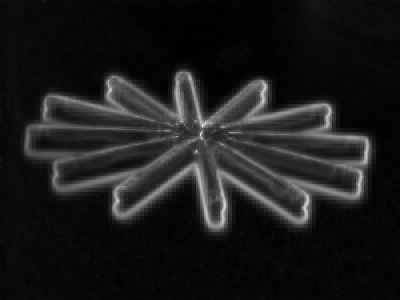
\includegraphics[width=0.7in,height=0.54in]{./Figures/contrast/1cont.jpg}
    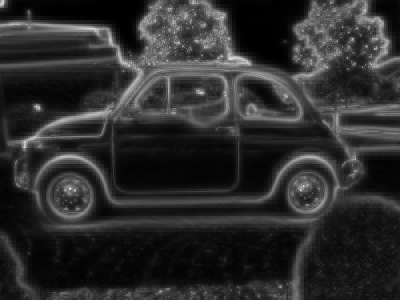
\includegraphics[width=0.7in,height=0.54in]{./Figures/contrast/2cont.jpg}
    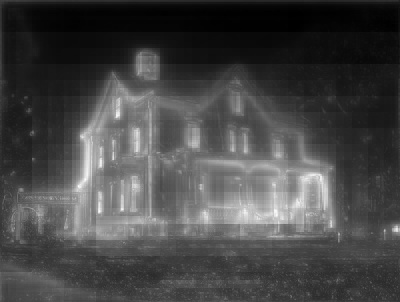
\includegraphics[width=0.7in,height=0.54in]{./Figures/contrast/3cont.jpg}
    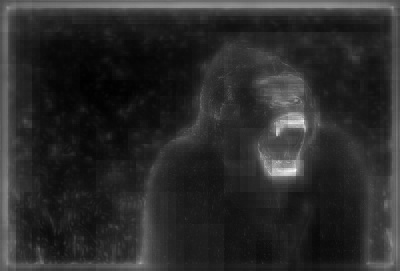
\includegraphics[width=0.7in,height=0.54in]{./Figures/contrast/4cont.jpg}\\
    \footnotesize \hspace{0.1cm} (a) \hs (b) \hs  (c) \hs (d) \\
\caption{Multiscale Contrast Feature Maps} \label{Fig:LocalFeatureMap}
    \end{center}
\end{figure}

Another disadvantage to only using multiscale contrast is that the inner regions of salient objects are poorly represented.  For example in the gorilla in Figure \ref{Fig:LocalFeatureMap}, the teeth are labelled as higher contrast to their surroundings compared to that of the body of the gorilla to the grass. Since each entry of the output feature map is quantitatively normalised, the contrast of the gorilla's body to the grass is rendered trivial compared to the contrast of the tooth. The tooth is not what the human receptive field would label as salient because it is a smaller part of the animal, and thus it should not be labelled as the salient object. This flaw may result in low recall comparing to the ground truth data when contrast is used as the sole method to distinguish a salient object.

\subsubsection{Centre-Surround Histogram}
%% regional feature

Multiscale contrast only partially detects salient objects, since it is only sensitive to the boundaries. In order to detect the object as a whole, we make use of another static salient feature which captures the regional information of an area, computed using various low-level features in a centre-surround difference calculation. 

To do this, we create a colour RGB histogram for both the rectangle and a surrounding frame with the same area as the rectangle, at a certain resolution (number of ``bins'' in the histogram). We then measure the difference between the area centred at each pixel $x$ and its surrounds by calculating the $\chi^2$ distance between the two histograms representative of those regions.  We do this for multiple aspect ratios $\{ 0.5, 0.75, 1.0, 1.25, 1.5\}$, and keep the largest (most distinct) $\chi^2$ value through the formula

\begin{align*}
R(x) &= \argmax\limits_{R(x)}\chi^2(R(x), R_s(x)) \\ &=\argmax\limits_{R(x)}\frac{1}{2}\cdot\SUM_{i\in bins}\frac{(hist_{R(x)_i}-hist_{R_s(x)_i})^2}{hist_{R(x)_i}+hist_{R_s(x)_i}}
\end{align*}

To reduce the computational complexity involved in this calculation, the size of the rectangle bounding the area in the centre is reduced to 12 discrete ratios $\{$0.18, 0.2, 0.25, 0.3, 0.35, 0.4, 0.45, 0.5, 0.55, 0.6, 0.65, 0.7, 0.75$\}$ with regards to  $min(w,h)$, the minimal value of width and height of the processed image.

The centre-surround histogram feature map at each pixel $x$ is output as $$f_h(x,I)\propto\SUM_{x'|x\in R(x')}w_{xx'}\chi^2(R(x'),R_s(x'))$$
This map reflects how distinct each pixel is from its surrounds, assigned from the largest $\chi^2$ value between the area centred at each pixel of the image and its surround, weighted by its spatial distance from the centre of that area. 

\begin{figure}[h]
    \begin{center}
    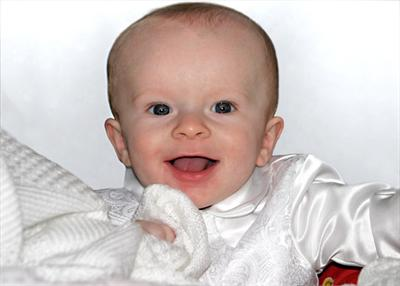
\includegraphics[width=0.7in,height=0.54in]{./Figures/CSH_image/1orig.jpg}
    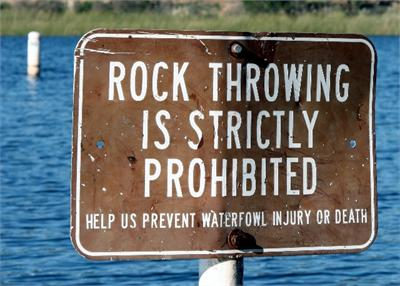
\includegraphics[width=0.7in,height=0.54in]{./Figures/CSH_image/2orig.jpg}
    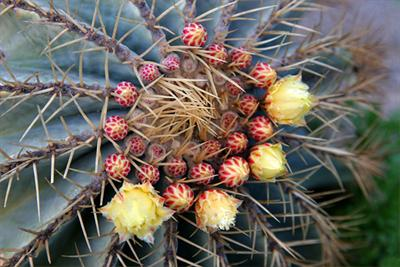
\includegraphics[width=0.7in,height=0.54in]{./Figures/CSH_image/3orig.jpg}
    \includegraphics[width=0.7in,height=0.54in]{./Figures/CSH_image/4orig.jpg}\\
    \includegraphics[width=0.7in,height=0.54in]{./Figures/CSH_image/1cont.jpg}
    \includegraphics[width=0.7in,height=0.54in]{./Figures/CSH_image/2cont.jpg}
    \includegraphics[width=0.7in,height=0.54in]{./Figures/CSH_image/3cont.jpg}
    \includegraphics[width=0.7in,height=0.54in]{./Figures/CSH_image/4cont.jpg}\\
    \footnotesize \hspace{0.1cm} (a) \hs (b) \hs  (c) \hs (d) \\
    \caption{Centre-Surrond Histogram Feature Maps} \label{Fig:RegionalFeatureMap}
    \end{center}
\end{figure}


As we can see from Figure \ref{Fig:RegionalFeatureMap}, the salient block within the image is given large emphasis comparing to its surrounds in the output feature map.  However, unlike multiscale contrast, the centre-surround histogram does not provide an accurate description of the boundary of the object -- an inherent drawback of this regional feature. Used together with the multiscale contrast map, the two features complement the other's weakness to create a stronger sense of the location of salient objects.

%% global feature
\subsubsection{Colour Spatial Distribution}

The goal of using colour spatial distribution is to take into account the global colour information in the image, that is, the information about how widely the colours occur in 
one image are distributed within it.  The computation of this feature is done in several parts.

First of all, we create a Gaussian mixture model with 5 components in order to capture relative colour distribution in the image. This can be represented as $\{c, \mu_c, \Sigma_c\}$ with regards to the colour component $c$ and fit of these components, making use of only a subset of pixels from the whole image. This is done to save on computational time required to process the feature, while at the same time not losing much accuracy as can be seen in \BOLD{FIG}.  We test three levels of pixel reduction via a Gaussian pyramid model: none, single-level reduction, and two-level reduction.  Single-level reduction halves the number of pixels used in creating the gaussian mixture model, whilst also providing a smoother distribution without sacrificing much accuracy.  The maximum number of iterations over the image is limited to 100 instances, and the convergence criterion is also lowered to $10^{-1}$ in order to reduce complexity without deteriorating the model.  Such simplification is possible only because the exact distribution is not required for capturing the approximate location of a salient object.

Using this model, each pixel is associated to a colour component with the probability $$P(c|I_x) = \frac{\omega_c\mathcal{N}(I_x|\mu_c,\Sigma_c)}{\SUM_c \omega_c \mathcal{N}(I_x|\mu_c,\Sigma_c)}$$where $\omega_c$ is the weight, $\mu_c$ is the mean colour, $\Sigma_c$ is the covariance, and $\mathcal N(I_x|\mu_c,\Sigma_c)$ is the multivariate normal distribution of the $c^{th}$ component. 

For each fitted gaussian colour component $c$, we compute its horizontal variance $V_{h}(c)$ as $$V_{h}(c) = \frac{1}{|X|_{c}} \sum_{x} p (c|I_{x}) \cdot | x_{h} - M_{h}(c) |^{2}$$where $x_h$ is horizontal coordinate of pixel $x$, $|X|_c$ is normalising factor and $M_h (c)$is the mean of the gaussian component$$|X|_c = \sum_x p(c|I_x)\\M_h (c) = \frac{1}{|X|_c} \sum_{x} p(c|I_x) \cdot x_h$$Its vertical variance $V_{v}(c)$ is defined similarly, and we combine the horizontal and vertical variances to derive the unnormalised composite variance $V_h (c)$:$$V' (c) = V_h (c) + V_v (c) $$

We then employ a min-max approach to normalise the composite covariance over the image$$V (c) = \frac{V'(c) - min \big(V'(c)\big) }{max \big(V'(c)\big) - min \big(V'(c)\big)}$$where $V(c)$ is the normalised composite covariance of the $c^{th}$ component, contained between 0 and 1.

Finally, due to the supposition that a salient object tends to have a less widely distributed colour, we set a penalty on the pixels which have a high variance colour. The ultimate colour spatial distribution feature for pixel $x$ is therefore defined as a weighted sum of its colour distribution $$f_s(x,I)\propto\SUM_c p(c|I_x)\cdot(1-V(c))$$

The feature map $f_s (\cdot,I)$ is normalized to the range $[0, 1]$. The following figure show colour spatial distribution feature maps over several images. The salient objects are labelled effectively by this global feature when there is a high distribution of other colours in the image.

\begin{figure}[h]
    \begin{center}
    \includegraphics[width=0.72in,height=0.52in]{./CSD_image/1.jpg}
    \includegraphics[width=0.72in,height=0.52in]{./CSD_image/2.jpg}
    \includegraphics[width=0.72in,height=0.52in]{./CSD_image/3.jpg}
    \includegraphics[width=0.72in,height=0.52in]{./CSD_image/4.jpg}\\
    \includegraphics[width=0.72in,height=0.52in]{./CSD_image/1_CSD.jpg}
    \includegraphics[width=0.72in,height=0.52in]{./CSD_image/2_CSD.jpg}
    \includegraphics[width=0.72in,height=0.52in]{./CSD_image/3_CSD.jpg} 
    \includegraphics[width=0.72in,height=0.52in]{./CSD_image/4_CSD.jpg} \\
    \footnotesize \hspace{0.1cm} (a) \hs (b) \hs  (c) \hs (d) \\
     \caption{Colour Spatial Distribution Feature Maps} \label{Fig:GlobalFeatureMap}
    \end{center}
\end{figure}

It is evident that the global feature gives a huge amount of accuracy to the detection algorithm when the background is monotonous, as illustrated by the first three images in Figure \ref{Fig:GlobalFeatureMap}. However, in the case of a varied and colourful background, the colour spatial distribution map fails to distinguish the salient object in the image. Figure \ref{Fig:GlobalFeatureMap} (d) demonstrates us this undesired property of the global feature. 

%One variation in our implementation is to create the component model from only a subset of the pixels in the image. The pixels in the subset is picked up with equal spatial distance. Specifically, we apply the "pydown" module in Opencv to dilute the pixels participating this unsupervised learning task. Such manipulation will not sacrifice too much accuracy, but greatly reduce  the running time of fitting the Mixture of Gaussians since the number of pixels provided for the fitting halves. 

\begin{figure}[h]
    \begin{center}
    \includegraphics[width=0.72in,height=0.52in]{./Figures/pydownCompare/1.jpg}
    \includegraphics[width=0.72in,height=0.52in]{./Figures/pydownCompare/1NOPYDOWN.jpg}
    \includegraphics[width=0.72in,height=0.52in]{./Figures/pydownCompare/1PYDOWN.jpg} 
    \includegraphics[width=0.72in,height=0.52in]{./Figures/pydownCompare/1DOUBLEPYDOWN.jpg} \\
    \includegraphics[width=0.72in,height=0.52in]{./Figures/pydownCompare/2.jpg}
    \includegraphics[width=0.72in,height=0.52in]{./Figures/pydownCompare/2NOPYDOWN.jpg}
    \includegraphics[width=0.72in,height=0.52in]{./Figures/pydownCompare/2PYDOWN.jpg} 
    \includegraphics[width=0.72in,height=0.52in]{./Figures/pydownCompare/2DOUBLEPYDOWN.jpg} \\
    \includegraphics[width=0.72in,height=0.52in]{./Figures/pydownCompare/3.jpg}
    \includegraphics[width=0.72in,height=0.52in]{./Figures/pydownCompare/3NOPYDOWN.jpg}
    \includegraphics[width=0.72in,height=0.52in]{./Figures/pydownCompare/3PYDOWN.jpg} 
    \includegraphics[width=0.72in,height=0.52in]{./Figures/pydownCompare/3DOUBLEPYDOWN.jpg} \\
    \footnotesize \hspace{0.1cm} (a) \hs (b) \hs  (c) \hs (d) \\
    \footnotesize (a) Original (b) No reduction (c) Single Level Reduction\\ (d) Two Level Reduction
    \caption{Example Colour Spatial Distributions on Reduced Pixels} \label{Fig:GlobalPydown}
    \end{center}
\end{figure}

%We test three levels of pixel dilution: no pydown, one-level pydown and two-level pydown. 
%One-level pydown means reducing both of the width and height of one image to half of the 
%original size,  such that only a quarter of pixels are available for fitting the mixture 
%of gaussians. From the above figure, it is evident that one-level pydown, to some extent, 
%increases the quality of  this global feature by marking the salient block softly or 
%obscurely rather than in a strict way. 

%Extraction for two-level pydown indicated in Fig.\ref{Fig:GlobalPydown} (d) is even faster, but generally 
%it lost the effectiveness of this global feature.

%Hence, in our implementation of color spatial distribution, we employ the one-level 
%pydown as a trick to both enhance quality of global feature and improve extraction time performance.


\newcommand{\bl}{\boldsymbol{\lambda}}
\newcommand{\bt}{\boldsymbol{t}}
\newcommand{\btx}{\boldsymbol{t}_x}
\newcommand{\bphix}{\boldsymbol{\phi}_x}

%% Learning (0.5 page)
\subsection{Learning}
The three features discussed beforehand all have strengths and weaknesses in different areas, however it goes without saying that adding them together provides an accurate description of the salient area in an image.  It would be over-simplistic to treat these features in equal weight since one feature may be better than the others at providing information about saliency. One effective and reasonable approach is to determine the optimal weight to combine three features with the help of a machine learning algorithm.  In this project, we implement logistic regression to decide the optimal weight on training data.

As mentioned before, the salient object detection is formulated as binary decision problem. From this perspective, we directly formulate the posterior distribution over the binary saliency variable $A_x$ as sigmoid function.
$$ y_x = p ( A_x = 1 | \bphix) = \frac{1}{1 + exp(-\bl \cdot \bphix)}$$
where the vector $\bphix$ contains three normalised energy $F_k (x, I)$ for each pixel $x$, and the parameter vector $\bl = \{ \lambda_1, \lambda_2, \lambda_3\}$ indicates how three extracted features form the unary term in the energy function utilised in the latter CRF inference.

Thus, the likelihood function of this whole image with given human label $\bt$ is
$$ p( \bt | \bl) = \prod_{x} y_{x}^{t_{x}} (1 - y_{x})^{1-t_x} $$
where the target variable $\bt$ is the ground truth map, and $\btx$ indicates the human-labelled binary saliency in the pixel $x$. 

We apply the maxmum likelihood estimation to evaluate the parameter $\bl$, based on the above likelihood function. Under this logistic regression framework, the ultimately learned parameter $\bl$ is $\{ \}$.
%% CRF Inference (0.5 - 1 page)
%% images for inferred binary mask
\subsection{CRF Inference}
The weighted unary potential made up from these weighted feature maps $$S_{unary}(a_x,I) = \SUM_{k=1}^K \lambda_k \cdot F_k(a_x,I)$$ is likely to already provide a good estimate of the salient area in the image.  However, to capture the spatial continuity of the salient area we infer the maximum likelihood assignment of pixel-wise variables under a conditional random field (CRF) framework.  A standard message-passing approach is infeasible when dealing with images at the pixel level, so we instead use $\alpha$-expansion inference, which successively segments all $\alpha$ and non-$\alpha$ pixels using graph cuts \cite{graphcut}.  The algorithm changes the value of $\alpha$ at each iteration using the graph cut algorithm; by this means, inferring the maximum likelihood assignment for each binary variable (or equivalently, the minimal energy function) is much faster. 

\begin{figure}[h]
\begin{center}
    \includegraphics[width=0.7in,height=0.48in]{./Figures/Lambda/5_145_145612.jpg}
    \includegraphics[width=0.7in,height=0.48in]{./Figures/Lambda/5_145_145612_2.jpg}
    \includegraphics[width=0.7in,height=0.48in]{./Figures/Lambda/5_145_145612_3.jpg} 
    \includegraphics[width=0.7in,height=0.48in]{./Figures/Lambda/5_145_145612_4.jpg} \\
    \includegraphics[width=0.7in,height=0.48in]{./Figures/Lambda/5_154_154292.jpg}
    \includegraphics[width=0.7in,height=0.48in]{./Figures/Lambda/5_154_154292_2.jpg}
    \includegraphics[width=0.7in,height=0.48in]{./Figures/Lambda/5_154_154292_3.jpg} 
    \includegraphics[width=0.7in,height=0.48in]{./Figures/Lambda/5_154_154292_4.jpg} \\
    \includegraphics[width=0.7in,height=0.48in]{./Figures/Lambda/5_154_154732.jpg}
    \includegraphics[width=0.7in,height=0.48in]{./Figures/Lambda/5_154_154732_2.jpg}
    \includegraphics[width=0.7in,height=0.48in]{./Figures/Lambda/5_154_154732_3.jpg} 
    \includegraphics[width=0.7in,height=0.48in]{./Figures/Lambda/5_154_154732_4.jpg} \\
    \footnotesize \hspace{0.1cm} (a) \hs (b) \hs  (c) \hs (d) \\
    \footnotesize  (a) Raw Image (b) $\lambda_0 = 1$  (c) $\lambda_0 = 10$ (d) $\lambda_0 =100$ \\
     \caption{Examples for Binary Mask with various Lambda $\lambda_0$}
\end{center}
\end{figure}


This requires a way to determine the parameter $\lambda_0$ which indicates to what extent, relative to the unary potential of the combined feature map, we ought to consider the pairwise potential in deciding the binary saliency of a pixel.  This parameter is key to influencing the smoothness of the resulting binary mask, since as discussed above it can be regarded as a penalty for labelling adjacent pixels with different values.

To determine a suitable $\lambda_0$, we apply cross validation at various magnitudes.  Using this, the optimal parameter $\lambda_0$ for calculating the final binary mask is $\lambda_0 = 8$.


\begin{figure}[h]
\begin{center}
    \includegraphics[width=0.8in,height=0.6in]{./Figures/CRFinference/5_159_159364.jpg}
    \includegraphics[width=0.8in,height=0.6in]{./Figures/CRFinference/5_159_159364_3.jpg}
    \includegraphics[width=0.8in,height=0.6in]{./Figures/CRFinference/5_159_159364_2.jpg} \\
    \includegraphics[width=0.8in,height=0.6in]{./Figures/CRFinference/5_159_159649.jpg}
    \includegraphics[width=0.8in,height=0.6in]{./Figures/CRFinference/5_159_159649_3.jpg}
    \includegraphics[width=0.8in,height=0.6in]{./Figures/CRFinference/5_159_159649_2.jpg} \\
    \includegraphics[width=0.8in,height=0.6in]{./Figures/CRFinference/5_162_162349.jpg}
    \includegraphics[width=0.8in,height=0.6in]{./Figures/CRFinference/5_162_162349_3.jpg}
    \includegraphics[width=0.8in,height=0.6in]{./Figures/CRFinference/5_162_162349_2.jpg} \\
    \footnotesize  (a) Raw Image (b) Combined Unary Map  (c) Binary Mask ($\lambda=8$)\\
     \caption{Examples for CRF inference by $\alpha$-expansion}
\end{center}
\end{figure}

%% Result evaluation in rectangle level (1 page)
%% images for the output rectangle
\section{Result Evaluation}
To evaluate our approach, we randomly pick 1000 images from the MSRA dataset B to form a training set.
We then choose another 500 images to form a testing set.

\subsection{Bounding Box}
The binary mask derived from the CRF inference can be used directly in a multitude of applications. However, in order to evaluate the accuracy of our approach, we make use of OpenCV's findContours algorithm \cite{topological} to output a bounding box rectangle around the detected salient object, based on the derived pixel-wise binary mask. The dimensions of this bounding box are written to a text file holding all resultant labels for that image directory.

\begin{figure}[h]
\begin{center}
    \includegraphics[width=0.6in,height=0.4in]{./Figures/boundingbox/5_145_145114RECT.jpg}
    \includegraphics[width=0.6in,height=0.4in]{./Figures/boundingbox/5_145_145275RECT.jpg}
    \includegraphics[width=0.6in,height=0.4in]{./Figures/boundingbox/5_145_145349RECT.jpg}
    \includegraphics[width=0.6in,height=0.4in]{./Figures/boundingbox/5_145_145398RECT.jpg}
    \includegraphics[width=0.6in,height=0.4in]{./Figures/boundingbox/5_146_146319RECT.jpg} \\
    \includegraphics[width=0.6in,height=0.4in]{./Figures/boundingbox/5_146_146330RECT.jpg}
    \includegraphics[width=0.6in,height=0.4in]{./Figures/boundingbox/5_146_146332RECT.jpg}
    \includegraphics[width=0.6in,height=0.4in]{./Figures/boundingbox/5_146_146431RECT.jpg}
    \includegraphics[width=0.6in,height=0.4in]{./Figures/boundingbox/5_146_146552RECT.jpg}
    \includegraphics[width=0.6in,height=0.4in]{./Figures/boundingbox/5_147_147367RECT.jpg} \\
    \includegraphics[width=0.6in,height=0.4in]{./Figures/boundingbox/5_148_148067RECT.jpg}
    \includegraphics[width=0.6in,height=0.4in]{./Figures/boundingbox/5_148_148271RECT.jpg}
    \includegraphics[width=0.6in,height=0.4in]{./Figures/boundingbox/5_148_148710RECT.jpg}
    \includegraphics[width=0.6in,height=0.4in]{./Figures/boundingbox/5_148_148763RECT.jpg}
    \includegraphics[width=0.6in,height=0.4in]{./Figures/boundingbox/5_148_148788RECT.jpg} \\
    \includegraphics[width=0.6in,height=0.4in]{./Figures/boundingbox/5_150_150590RECT.jpg}
    \includegraphics[width=0.6in,height=0.4in]{./Figures/boundingbox/5_151_151334RECT.jpg}
    \includegraphics[width=0.6in,height=0.4in]{./Figures/boundingbox/5_153_153455RECT.jpg}
    \includegraphics[width=0.6in,height=0.4in]{./Figures/boundingbox/5_153_153651RECT.jpg}
    \includegraphics[width=0.6in,height=0.4in]{./Figures/boundingbox/5_154_154297RECT.jpg} \\
    \includegraphics[width=0.6in,height=0.4in]{./Figures/boundingbox/5_155_155096RECT.jpg}
    \includegraphics[width=0.6in,height=0.4in]{./Figures/boundingbox/5_155_155145RECT.jpg}
    \includegraphics[width=0.6in,height=0.4in]{./Figures/boundingbox/5_155_155333RECT.jpg}
    \includegraphics[width=0.6in,height=0.4in]{./Figures/boundingbox/5_155_155196RECT.jpg}
    \includegraphics[width=0.6in,height=0.4in]{./Figures/boundingbox/5_155_155459RECT.jpg} \\
    \caption{Examples images for bounding box output}
\end{center}
\end{figure}

% TODO add some analysis here.

\subsection{Evaluation Criteria}
%% why we need evaluation criteria
%The main functionality of evaluation criteria is to measure the effectiveness of our approach.
%In our project, evaluation will be applied, as well, in the cross validation while determining the 
%energy function parameter $\lambda_0$. 
%But what kind of criteria could effectively capture the goodness of our model?
As to this project, we utilise the both approaches to evaluate our result:
region-based and boundary-based measurements.

\subsubsection{Region-based measurement}
Precision and Recall both take significant roles in the information retrieval as a performance indicator.  They are used in this project in evaluating the correctness of the output rectangle.

The precision represents the percentage of pixels that are correctly detected in ground truth, which is the ratio of the number of pixels in overlapped region to pixel number contained in the ground truth box. The recall reflects the percentage of pixels that are correctly detected in resulted detection, which is the ratio of pixel number the overlapped region contained to the number of pixels.
%% explain what is by graph and diagram

\begin{figure}[h]
\begin{center}
    \includegraphics[width=1.0in,height=0.8in]{Figures/Creteria/B.jpg}
    \includegraphics[width=1.0in,height=0.8in]{Figures/Creteria/C.jpg} 
    \includegraphics[width=1.0in,height=0.8in]{Figures/Creteria/A.jpg} \\
    \footnotesize (a) \hs \hspace*{0.8cm} (b)  \hs \hspace*{0.8cm} (c)
    \caption{Examples with resulted detection and ground truth} \label{Fig:PrecisionANDRecall}
    \footnotesize Red Box: ground truth label. Green Box: detected label.
\end{center} \end{figure}

It is evident that all three results in Figure \ref{Fig:PrecisionANDRecall} are far from satisfying. The salient detection in the leftmost image has high precision but the recall is very low, meaning that it has failed to detect all truly salient pixels.  The middle image is no better, with high recall but low precision, with a saliency leak into the surrounding region.

For an overall performance measurement, the F-measure indicator is suitable, with $\alpha = 0.5$ giving the weighted harmonic mean of precision and recall:$$F_{0.5} = \frac{1.5\times Precision \times Recall}{ 0.5 \times Precision + Recall}$$

\subsubsection{Boundary-based measurement}
Boundary Displacement Error (BDE) measures the average of positional difference of ground truth and resulted detection.  It does this by calculating the average minimum Euclidian distance between the set of pixels in one label $B_1$ and each pixel $x$ in the other label $B_2$ \cite{bde} $$BDE(B_1,B_2)=\frac{\SUM_{x\in B_1}\min\limits_{y\in B_2}\{d_E(x,y)\}}{|B_1|}$$  A perfect score is 0, where every point in the result output label is contained in the set of points in the truth label.  As the results differ more and more from the ground truth, the average BDE value becomes higher.

\subsection{Results and Discussion}
The average BDE score for our algorithm is \BOLD{ACTUALSCORE}, which is based on training and test sets from the MSRA dataset B.  We were not able to calculate the F-measure for performance.

Part of the reason for this somewhat low score is that the contours around the saliency mask map are not always fully closed, leading to high precision with a bounding box rectangle around a single point since it is the largest discovered closed area.  Creating a bounding box around all salient points in an image has the opposite effect, with a large recall but multiple non-salient areas of the image contained within the bounding box because of small areas where a ``saliency leak'' has occurred.

%% Discussion (existing flaws and possible improvements) (0.5 page)
\section{Conclusion}
In this project, we have demonstrated a supervised approach for salient object detection, formulated as a binary labelling problem using a set of local, regional, and global salient object features.  However, there is much room for improvement, especially in the labelling of the salient areas from the derived binary mask.  There is also a lack of comparison with other methods using numerical evaluations, which may demonstrate greater effectiveness of the approach in this report.

There are still several remaining issues for further investigation.  These include the ability to detect multiple salient areas in an image, improving on previous and current work to form a computational model capable of describing a scene.  Another application could be in real-time detection for use in robotics and recording or playback applications.  Failure cases can be remedied by creating a more adept algorithm that captures the closest 98\% of salient pixels, resulting in much higher accuracy overall.  There may also be better ways to derive a label from the raw binary mask of an image to pursue.

%\cite{drwn}\cite{sal2007}\cite{sal2011}\cite{itti}\cite{ittiphd}\cite{graphcut}\cite{topological}\cite{fuzzy}

%% acknowlegement and reference (0.5 page)
\bibliographystyle{ieee}
\bibliography{main}

%\begin{thebibliography}{99} \fontsize{9pt}{50} \setlength{\itemsep}{-0.5pt} 
%    \bibitem 1 Liu, Tie, et al. "Learning to detect a salient object." 
%        \textit{Computer Vision and Pattern Recognition, 2007. CVPR07. IEEE Conference on. IEEE, 2007}.
%
%    \bibitem 2 Liu, Tie, et al. "Learning to detect a salient object." 
%        \textit{Pattern Analysis and Machine Intelligence, IEEE Transactions on 33.2 (2011): 353-367}. 
%
%    \bibitem 3 Itti, Laurent, Christof Koch, and Ernst Niebur. "A model of saliency-based visual attention for rapid scene analysis."
%        \textit{Pattern Analysis and Machine Intelligence, IEEE Transactions on 20.11 (1998): 1254-1259}.
%
%    \bibitem 4 Ma, Yu-Fei, and Hong-Jiang Zhang. "Contrast-based image attention analysis by using fuzzy growing."
%        \textit{ Proceedings of the eleventh ACM international conference on Multimedia. ACM, 2003}. 
%
%    \bibitem 5 L. Itti. Models of Bottom-Up and Top-Down Visual Attention. PhD thesis, 
%        \textit{California Institute of Technology Pasadena, 2000}.
%
%    \bibitem 6 Boykov, Yuri, Olga Veksler, and Ramin Zabih. "Fast approximate energy minimization via graph cuts." 
%        \textit{Pattern Analysis and Machine Intelligence, IEEE Transactions on 23.11 (2001): 1222-1239}.
%
%    \bibitem 7 Suzuki, S. and Abe, K., Topological Structural Analysis of Digitized Binary Images by Border Following. 
%        \textit{CVGIP 30 1, pp 32-46 (1985)}.
%
%    \bibitem 8 Gould, Stephen. "DARWIN: A Framework for Machine Learning and Computer Vision Research and Development." 
%        \textit{Journal of Machine Learning Research 13 (2012): 3533-3537}.
%
%\end{thebibliography}
%-------------------------------------------------------------------------

\end{document}
